% Created 2013-12-20 金 04:52
\documentclass[12pt]{jsarticle}
\usepackage[dvipdfmx]{graphicx}
\usepackage{comment}
%\usepackage{setspace}
%%\date{\today}
%\title{}
\textheight = 25truecm
\textwidth = 18truecm
\topmargin = -1.5truecm
\oddsidemargin = -1truecm
\evensidemargin = -1truecm
\marginparwidth = -1truecm
\def\theenumii{\Alph{enumii}}
\def\theenumiii{\alph{enumiii}}
\def\labelenumi{(\theenumi)}
\def\labelenumiii{(\theenumiii)}
%\setstretch{0.9}
\begin{document}

%\maketitle
%\tableofcontents

\begin{center}
%%%%%%%%%%%%%%%%%%%%%%%%%%%%%%%%%%%%%%%
%%%タイトル                         %%%
%%%%%%%%%%%%%%%%%%%%%%%%%%%%%%%%%%%%%%%
{\LARGE NICドライバの改変すべき箇所の調査}
\end{center}

\begin{flushright}
  2014/10/16\\
  藤田将輝
\end{flushright}
%%%%%%%%%%%%%%%%%%1章%%%%%%%%%%%%%%%%%%%
\section{はじめに}

NICなしでNICのデバイスドライバの割り込みハンドラを動作させ,パケット受信処理をさせるため,
NICドライバの改変箇所を調査している.
本資料ではこの調査内容を示す.


\section{目標: 本機構におけるNICドライバの受信割り込みの処理流れ}
本機構の目標であるNICドライバの受信割り込みの処理流れを図1に示し,以下で説明する.
\begin{enumerate}
\item 割り込み情報の指定\\
プログラマが割り込みジェネレータを用いて割り込み情報を指定する.
\item 割り込み情報の通知\\
割り込みジェネレータから割り込み元OSのデバッグ支援機構へ割り込み情報を通知する.
\item パケットの生成\\
割り込み元OSのデバッグ支援機構がパケットを生成する.
\item 受信バッファへのパケットの格納\\
割り込み元OSのデバッグ支援機構が受信バッファへパケットを格納する.
\item 受信バッファ状態の更新\\
割り込み元OSのデバッグ支援機構が受信バッファ状態を受信済み状態に更新する.
\item 割り込み発生要求\\
割り込み情報をもとに,割り込み元OSのデバッグ支援機構からコア0へ割り込み発生要求を行う.
\item IPIの送信\\
割り込み元OSが保持するコア0から割り込み先OSが保持するコア1へIPIを送信する.
\item 割り込み処理の開始\\
割り込み先OSが割り込み処理を開始する.この際,割り込み先OSが割り込みベクタ番号に対応した割り込みハンドラ
を実行する.
\item 受信バッファの特定\\
受信ディスクリプタが保持する受信バッファ状態をデバッグ対象OSのNICドライバが参照する.
これにより,パケットが格納されている受信バッファを特定する.
\item ソケットバッファへのパケットの格納\\
受信バッファからソケットバッファへデバッグ対象OSのNICドライバがパケットを格納する.
\end{enumerate}


\begin{figure}[t]
\begin{center}
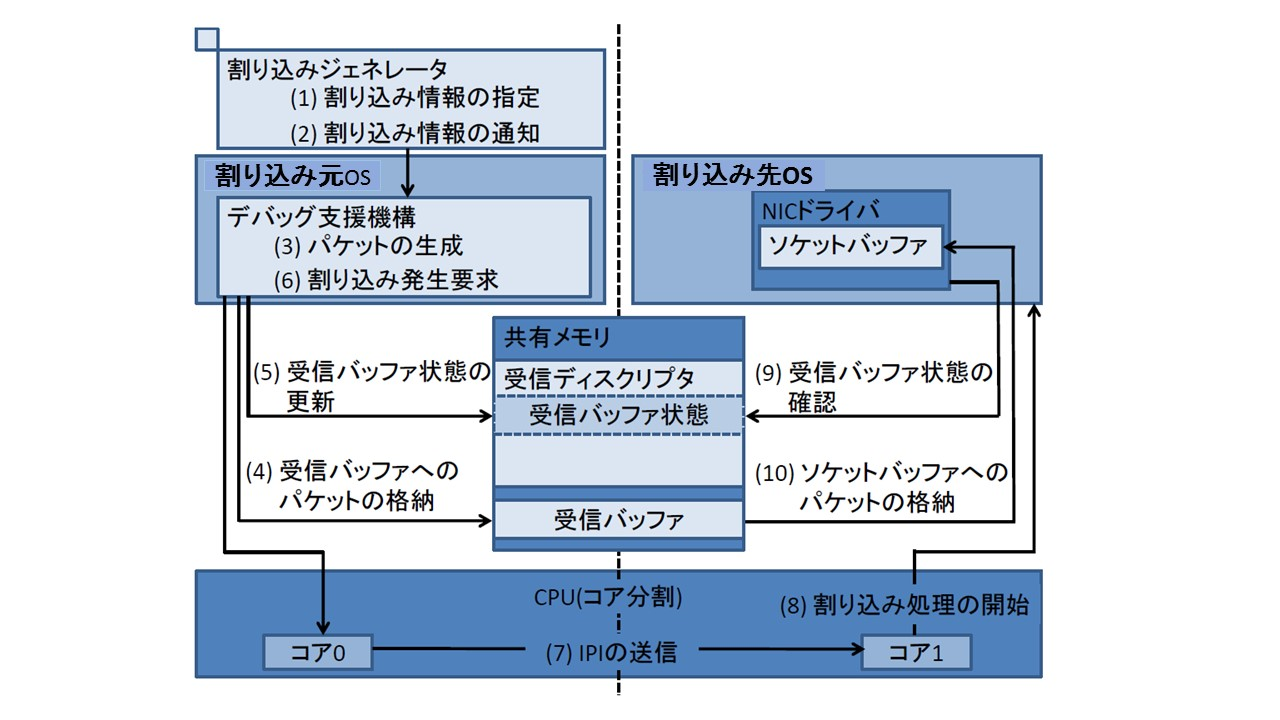
\includegraphics[height=8.0cm]{./fig1.jpg}          
\caption{NICドライバへの割り込み挿入の流れ}
\label{fig:up}
\end{center}
\end{figure}






\section{NICドライバを改変することで実現する機能}
前章で述べた流れのうち,NICドライバを改変し,共有メモリを使用することによって(8)(9)(10)を実現する.
具体的には割り込み先OSの占有するコアがIPIを受信すると動作する割り込みハンドラで
NICのデバイスドライバのパケット受信処理に関する関数を呼び出せるようにする.
また,受信バッファの特定先をMintの共有メモリに変更し,
Mintの共有メモリ上に作成してある擬似的な受信バッファからNICドライバのソケットバッファへデータを転送可能にする.

\section{改変すべき箇所}
2章の(8)(9)(10)の
それぞれについての対処を以下に述べる.
\begin{description}
\item[【(8)の対処】]\mbox{}\\
割り込み先OSがIPIを受信すると動作する割り込みハンドラとして
改変したNICのデバイスドライバの関数を呼び出すハンドラを登録する.
\item[【(9)の対処】]\mbox{}\\
受信バッファを特定する際のアドレスをMintの共有メモリ上に作成した擬似的な受信バッファのアドレスに変更する.
\item[【(10)の対処】]\mbox{}\\
(9)の対処により,Mintの共有メモリ上に作成した擬似的な受信バッファからデバイスドライバのソケットバッファに
パケットを格納する.
\end{description}


\section{おわりに}
本資料では本機構における最終目標と,これを実現するためのNICドライバの改変箇所について述べた.
今後は具体的な関数の調査と,改変によって発生しうる問題点の調査,NICドライバの改変を行う.
\end{document}
